\section{Preliminaries}\label{sect:backgrRegex}
We start by recalling the notion of regular expressions over finite words. 
Since, as it will be clear later, we are interested in expressing requirements 
over finite words over $2^{\Prop}$, here we consider \emph{proposition-based} 
%\emph{propositional-based} 
regular expressions (denoted as $\RE$s), where atomic expressions are 
propositional (Boolean) formulas over $\Prop$, instead of just letters over an 
alphabet. Formally, the set of $\RE$s $r$ over $\Prop$ is defined by the 
grammar:
%
\[
    r ::= \varepsilon\;\vert\; \phi\;\vert\; r\cup r\;\vert\; r\cdot r\;\vert\; r^{*},
\]
where $\phi$ is a propositional formula over $\Prop$. The length $|r|$ of an $\RE$ $r$ is the number of subexpressions of $r$.
 An $\RE$ $r$ denotes a language $\Lang(r)$ of finite words over $2^{\Prop}$ defined as:
\begin{itemize}
  \item $\Lang(\varepsilon)=\{\varepsilon\}$,
  \item $\Lang(\phi)=\{A\in 2^{\Prop}\mid A \text{ satisfies }\phi\}$,
  \item $\Lang(r_1\cup r_2)=\Lang(r_1)\cup \Lang(r_2)$,
  \item $\Lang(r_1\cdot r_2)=\Lang(r_1)\cdot \Lang(r_2)$, 
\item $\Lang(r^{*})=(\Lang(r))^{*}$.
\end{itemize}
By well-known results,  the class of $\RE$ over $\Prop$ captures the class of regular languages of finite words over $2^{\Prop}$.

\begin{example}\label{example:re}
An example of  $\RE$ is $r_1=\mathbf{(p\wedge s)} \cdot \mathbf{s}^* \cdot \mathbf{(p\wedge s)}$ that intuitively denotes the set of finite words where both $\mathbf{p}$ and $\mathbf{s}$ hold true on the endpoints, and $\mathbf{s}$ continuously holds in all internal symbols/sets of $2^{\Prop}$. The $\RE$ $r_2=\mathbf{(\neg p)}^*$ denotes the set of finite words such that $\mathbf{p}$ does not hold in any position.
\end{example}

We also recall the standard notion of
\emph{non-deterministic finite state automaton} ($\NFA$), which is a tuple 
$\Au =\tpl{\Sigma,Q,Q_0,\Delta,F}$, where $\Sigma$ is a finite alphabet, $Q$ is a finite set of states, $Q_0\subseteq Q$ is the set of initial states,
$\Delta: Q\times \Sigma \to  2^Q$ is the transition function (or, equivalently, 
$\Delta\subseteq Q\times \Sigma \times Q$), and $F\subseteq Q$ is the set of 
accepting states. 
An $\NFA$ $\Au$ is \emph{complete} if, for all $(q,\sigma)\in Q\times \Sigma$, $\Delta (q,\sigma)\neq \emptyset$.
Given a finite word $w$ over $\Sigma$, with $|w|=n$, and two states $q,q'\in 
Q$, a \emph{run} (or \emph{computation}) of $\Au$ from $q$ to $q'$ over $w$ is 
a finite sequence of states $q_1,\ldots,q_{n+1}$ such that $q_1=q$, 
$q_{n+1}=q'$, and $q_{i+1} \in \Delta(q_i,w(i))$ for all $i\in [1,n]$. The 
language $\Lang(\Au)$  \emph{accepted by} $\Au$ consists of the set of  finite 
words $w$ over $\Sigma$ such that there is a run over $w$ from some initial 
state to some accepting state.

A \emph{deterministic finite state automaton} ($\DFA$) is an $\NFA$ $\Du=\tpl{\Sigma,Q,Q_0,\Delta,F}$ such that $Q_0$ is a singleton, and for all $(q,c)\in Q\times \Sigma$, $\Delta(q,c)$ is a singleton. In the following, in the case of a $\DFA$, we will denote the transition function $\Delta$ as $\delta$.

\begin{remark}\label{remk:nfa}
By well-known results, given an $\RE$ $r$ over $\Prop$, one can construct, in a compositional way, an $\NFA$ $\Au_r$ with alphabet $2^{\Prop}$, whose number of states is at most $2|r|$, such that $\lang(\Au_r) = \lang(r)$. 
%Moreover, the construction is compositional and the automata associated with two $\RE$ $r$ and $r'$ share the states associated with the common subexpressions of $r$ and $r'$.
We call $\Au_r$ the \emph{canonical} $\NFA$ associated with $r$. 

Note that, though the number of edges of $\Au_r$ may be exponential in $|\Prop|$ (edges are labelled by assignments $A\in 2^\Prop$
satisfying propositional formulas $\phi$ of $r$), we can avoid explicitly 
storing edges, as they can be recovered in polynomial time from $r$. 

In  
Figure~\ref{fig:NFAex}, we depict the canonical $\NFA$ $\Au_{r_1}$ associated 
with the $\RE$ $r_1$ of  Example~\ref{example:re}.
We can avoid storing the edges of $\Au_{r_1}$ by remembering which propositional formulas of $r_1$ they are associated with.

\begin{figure}[H]
\centering
\begin{tikzpicture}[->,>=stealth',shorten >=1pt,auto,node distance=2.8cm,
                    semithick]
  %\tikzstyle{every state}=[fill=red,draw=none,text=white]
  \node[state] 		(A) 			 {$q_0$};
  \node[state]         		(B) [right of=A] {$q_1$};
  \node[accepting,state]    (D) [right of=B] {$q_2$};
  \node[draw=none] 			(Z) [above of=A, yshift=-1.5cm] {$\mathcal{A}_{r_1}$};

  \path (A) edge              node {$\mathbf{(p\wedge s)}$} 	(B)
        (B) edge [loop above] node {$\mathbf{s}$} 			(B)
        (B) edge              node {$\mathbf{(p\wedge s)}$} 	(D);
\end{tikzpicture}
\caption{The canonical $\NFA$ $\Au_{r_1}$ associated with the $\RE$ $r_1$ of Example~\ref{example:re}.
%We can avoid storing the edges of $\Au_{r_1}$ by remembering which propositional formulas of $r_1$ they are associated with.
}\label{fig:NFAex}
\end{figure}
\end{remark}

In the previous chapters, $\HS$ formulas are evaluated over intervals which correspond to the traces of a Kripke structure $\Ku$. The approach followed is subject to two restrictions: $(i)$ the set of  proposition letters of $\HS$ formulas and the set $\Prop$ of proposition letters of the  Kripke structure
coincide, and $(ii)$ a proposition letter holds over an interval if and only if it holds over all its sub-intervals (\emph{homogeneity assumption}). 
%
Here we adopt a more general and expressive approach.

Let $\mathpzc{P}_u$ be a finite set of \emph{abstract (uninterpreted) interval properties}.
An abstract interval property $p_u\in \mathpzc{P}_u$ denotes a regular language of finite words over $2^{\Prop}$.
More specifically,
every $p_u$ is a proposition-based regular expression over $\Prop$,
and it \emph{occurs as a proposition letter} in $\HS$ formulas. 
Thus, hereafter, an \HS\ formula $\varphi$ over $\Prop$ is an $\HS$ formula whose proposition letters (i.e., atomic formulas) are $\RE$s $r$ over $\Prop$.
%
For this reason, we define
the size (or length) $|\varphi |$ of $\varphi$ as the number of non-atomic subformulas of $\varphi$ plus $\sum_{r\in \SPEC} |r|$, where $\SPEC$ is the set of $\RE$s occurring in $\varphi$. 

We now define the semantics of an \HS\ formula $\varphi$ over $\Prop$ on a 
trace $\rho$ of a (finite) Kripke structure $\Ku=\KuDef$.
For the purpose we need the following definition.
\begin{definition}[Labelling sequence induced by a trace]
 A trace $\rho\in\Trk_\Ku$, with $|\rho|=n$, induces a finite word over $2^{\Prop}$, denoted as $\mu(\rho)$ and called \emph{labeling sequence}, defined as \[\mu(\rho(1))\cdots \mu(\rho(n)).\]
\end{definition}
Now, the satisfaction relation $\Ku,\rho\models \varphi$ can be defined inductively as follows (we omit the standard clauses for Boolean connectives):
\begin{itemize}
    \item $\Ku,\rho   \models r$ if and only if $ \mu(\rho) \in \Lang(r)$ for each $\RE$ $r$ over $\Prop$,
    \item $\Ku,\rho  \models \hsB\varphi$ if and only if there exists $\rho'\in\Pref(\rho)$ such that $\Ku,\rho' \models \varphi$,
    \item $\Ku,\rho  \models \hsE\varphi$ if and only if there exists $\rho'\in\Suff(\rho)$ such that $\Ku,\rho' \models \varphi$,
    \item $\Ku,\rho   \!\models\! \hsBt\varphi$ if and only if $\Ku,\rho'   \!\models\! \varphi$ for some trace $\rho'$ such that $\rho\!\in\!\Pref(\rho')$, 
    \item $\Ku,\rho   \!\models\! \hsEt\varphi$ if and only if $\Ku,\rho'   \!\models\! \varphi$ for some trace $\rho'$ such that $\rho\!\in\!\Suff(\rho')$. 
\end{itemize} 

As in the previous chapters, 
we say that $\Ku$ is a \emph{model} of $\varphi$, denoted as $\Ku\models 
\varphi$, if, for all \emph{initial} traces $\rho$ of $\Ku$, it holds that 
$\Ku,\rho\models \varphi$. The \emph{MC problem} for $\HS$ is the problem of 
checking, given a finite Kripke structure $\Ku$ and an $\HS$ formula $\varphi$, 
whether or not $\Ku\models \varphi$. Again, the problem is not trivially 
decidable since the set $\Trk_\Ku$ of traces of $\Ku$ is infinite.

With reference to Chapter~\ref{chap:TOCL17}, we recall that
the considered \emph{state-based semantics} provides a \emph{branching-time 
setting both in 
the past and in the future}. In particular, while modalities for $\hsB$ and 
$\hsE$ are linear-time (as they allow us to select prefixes and suffixes of the 
current trace only), modalities for $\hsA$ and $\hsBt$ (respectively, $\hsAt$ 
and $\hsEt$) are branching-time in the future (respectively, in the past) since 
they enable us to nondeterministically extend a trace in the future 
(respectively, in the past). 

As shown in Chapter~\ref{chap:TOCL17}, under the 
considered semantic version, the logics $\HS$ and $\CTLStar$ are expressively 
incomparable already under the homogeneity assumption. However, under such an 
assumption, the use of  the past branching-time modalities $\hsAt$ and $\hsEt$ 
is necessary for capturing requirements which cannot be expressed in 
$\CTLStar$. For instance, the constraint
``\emph{each state reachable from the initial one where $p$ holds has a 
predecessor where $p$ holds as well}'' cannot be expressed in \CTLStar, but can 
be easily stated in the fragment $\AbarE$ (see Section~\ref{sect:allSems}). 

Conversely, in the more expressive  setting based on regular expressions, the future branching-time modalities $\hsA$ and $\hsBt$ are already sufficient for capturing requirements which cannot be expressed in \CTLStar, such as the following branching-time bounded response property: ``\emph{for each state reachable from the initial one, where a request  $\emph{req}$ occurs, there is a computation starting from this state such that the request is followed by a response $\emph{res}$ after an  \emph{even number} of steps}''. This requirement can be expressed in the  fragment $\ABbar$ as follows: 
\[\hsAu(\text{req} \rightarrow \hsBt (\text{req}\cdot (\top\cdot \top)^{*}\cdot \text{res})).\] 
Note that it says nothing about the possible occurrence of a response 
$\emph{res}$ after an \emph{odd} number of steps.

Before moving on, we show that
in this setting it is easy to force homogeneity: we just have to impose that 
all 
regular expressions in the formula have the form $p\cdot p^*$, for some 
$p\in\Prop$.
Additionally, labelling of 
intervals by endpoints can be easily captured by regular expressions having the form:
\[\bigcup_{(i,j)\in I} (q_i\cdot \top^*\cdot q_j)\cup\bigcup_{i\in I'} q_{i},\]
for some suitable sets of indexes $I\subseteq \{1,\ldots,|S|\}^2$ and 
$I'\subseteq \{1,\ldots,|S|\}$, where $q_i\in\Prop$ is a letter labeling the 
state $s_i\in S$ of $\Ku$, only.

\begin{example}[Adapted from \cite{lm16}]
With this (toy) example we want to compare the effectiveness of regular expressions as rules for defining interval labelling, to homogeneity and to endpoint-based labelling.

In Figure~\ref{fig:printing}, a Kripke structure representing a printer is shown.
In $\sinit$ the printer starts printing a sheet; in $s_1$ the process is ongoing, and it ends in $s_2$. The printer then prints the subsequent sheet, by \lq\lq moving\rq\rq{} back to $\sinit$.

Imagine we want to label the process of printing a \emph{single sheet} by $p$ (i.e., only the trace $s_0s_1s_2$).
Under homogeneity, if $s_0s_1s_2$ is labeled by $p$, then $s_0$, $s_1$, $s_2$, $s_0s_1$, $s_1s_2$ must be all labeled by $p$ as well, against our idea.
In the endpoint-based approach, in order for $p$ to label $s_0s_1s_2$, $p$ must also label all traces $(s_0s_1s_2)^n$ for $n\in \Nat^+$, as the endpoints of all these are $s_0,s_2$. Thus \lq\lq several, consecutive sheets\rq\rq{} are labelled $p$.

Conversely, we just write the proposition-based $\RE$ $\mathbf{p_\text{st}} \cdot ( \mathbf{\neg p_\text{end}\wedge \neg p_\text{st}})^* \cdot \mathbf{p_\text{end}}$ to capture precisely the trace $s_0s_1s_2$.

\begin{figure}[H]
    \centering
    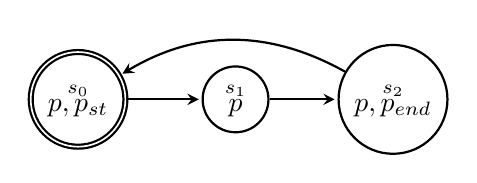
\begin{tikzpicture}[->,>=stealth,thick,shorten >=1pt,auto,node distance=2cm,every node/.style={circle,draw}]
		\node [style={double}](v0) {$\stackrel{s_0}{p,p_\text{st}}$};
		\node (v1) [right of=v0] {$\stackrel{s_1}{p}$};
		\node (v2) [right of=v1] {$\stackrel{s_2}{p,p_\text{end}}$};

		\draw (v0) to (v1);
		\draw (v1) to (v2);
		\draw (v2) to [bend right] (v0);
		\end{tikzpicture}
    \caption{Kripke structure representing a printer}
    \label{fig:printing}
\end{figure}
\end{example}
